\section{Nghiên cứu siêu tham số}

Mục này so sánh ba cấu hình siêu tham số có kiểm soát, mỗi cấu hình chỉ thay đổi đúng một yếu tố so với baseline để cô lập nguyên nhân. Cấu hình đầu nâng learning rate lên gấp năm lần baseline ($\eta = 5 \times 10^{-3}$) nhằm khảo sát điểm gãy giữa hội tụ nhanh và dao động/divergence trên động học hồi quy. Cấu hình thứ hai giảm learning rate xuống một phần năm baseline ($\eta = 2 \times 10^{-4}$) để khảo sát mặt còn lại của đánh đổi, giữa tốc độ hội tụ chậm và độ tổng quát hóa tốt hơn nhờ noise SGD path nhỏ hơn. Cấu hình thứ ba tăng batch size lên $256$ trong khi giữ nguyên learning rate, qua đó chủ động bộc lộ trade-off mà lý thuyết tỷ lệ tuyến tính (\textit{linear scaling rule}) đã chỉ ra: gradient có ít nhiễu hơn nhưng số bước cập nhật trong một epoch ít hơn bốn lần, khiến hội tụ tổng thể chậm lại nếu learning rate không được nhân lên tương ứng.

Kết quả ba epoch đầu của ba cấu hình được tổng hợp ở Bảng~\ref{tab:so-sanh-sieu-tham-so}, cùng với baseline năm epoch để đối chiếu.

% Nhớ thêm \usepackage{tabularx} và \usepackage{booktabs} vào file main.tex
\begin{table}[htbp]
\centering
\caption{Kết quả so sánh siêu tham số trên tập validation.}
\label{tab:so-sanh-sieu-tham-so}
\begin{tabularx}{\textwidth}{l c c >{\centering\arraybackslash}X >{\centering\arraybackslash}X >{\centering\arraybackslash}X}
\toprule
\textbf{Cấu hình} & \textbf{Learning rate} & \textbf{Batch size} & \textbf{Val loss tốt nhất} & \textbf{Val accuracy tốt nhất} & \textbf{Epoch tới điểm tốt nhất} \\ \midrule
Baseline          & $10^{-3}$              & 64                  & 0,3042                     & 0,8776                         & 3                                \\ \addlinespace
LR cao            & $5 \times 10^{-3}$     & 64                  & 0,2900                     & 0,8928                         & 2                                \\ \addlinespace
LR thấp           & $2 \times 10^{-4}$     & 64                  & 0,3071                     & 0,8736                         & 2                                \\ \addlinespace
BS lớn            & $10^{-3}$              & 256                 & 0,3469                     & 0,8680                         & 3                                \\ \bottomrule
\end{tabularx}
\end{table}

Hình~\ref{fig:duong-cong-sieu-tham-so} trực quan hóa đường cong validation loss và validation accuracy theo epoch cho ba cấu hình thí nghiệm, cho phép quan sát tốc độ hội tụ và độ ổn định của từng cấu hình.

\begin{figure}[htbp]
    \centering
    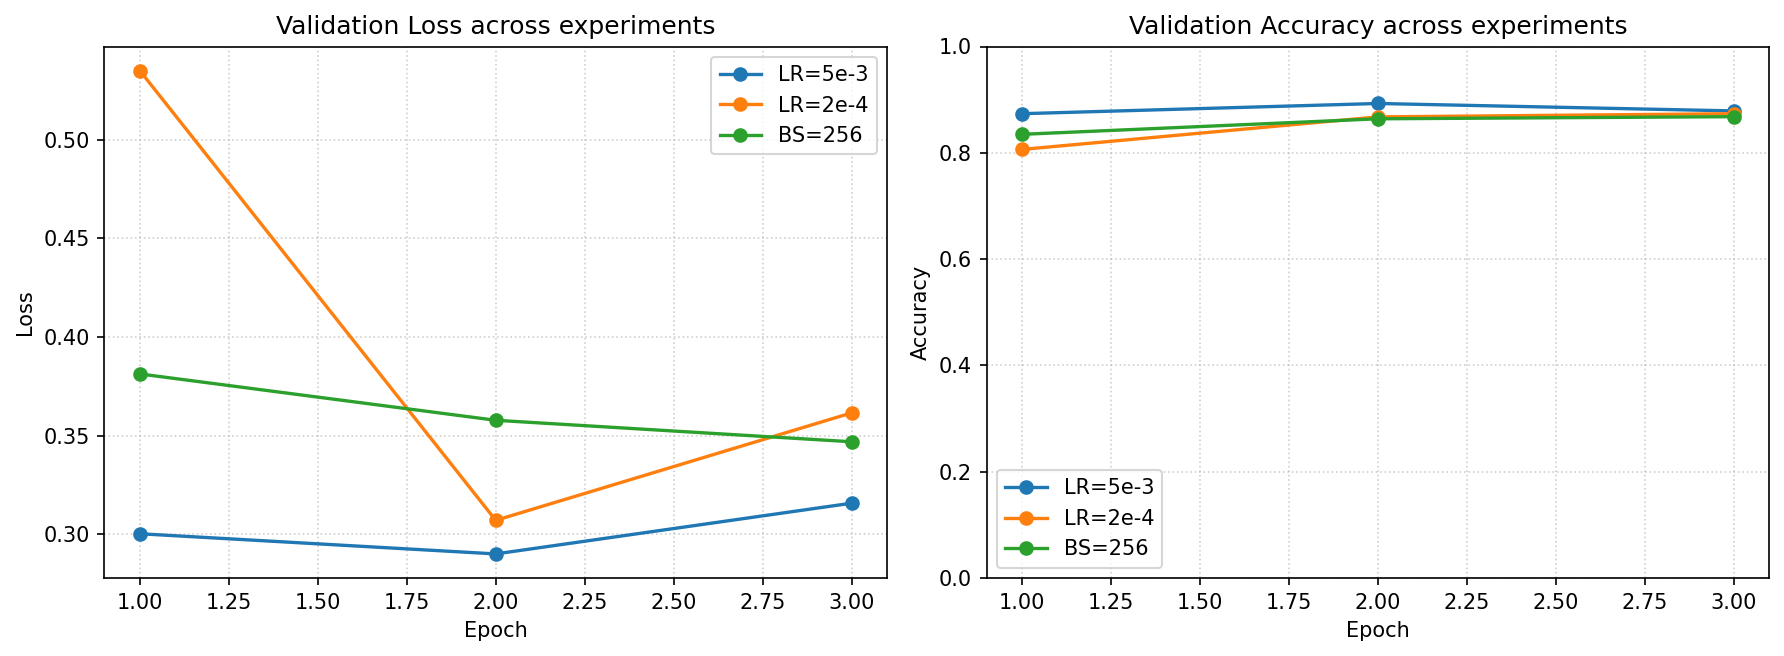
\includegraphics[width=0.9\textwidth]{figures/experiment_comparison.png} % Điền đường dẫn ảnh đồ thị của bạn ở đây
    \caption{So sánh val loss (trái) và val accuracy (phải) qua các epoch giữa
ba cấu hình thí nghiệm.}
    \label{fig:duong-cong-sieu-tham-so}
\end{figure}

Quan sát đáng chú ý nhất là cấu hình LR cao đạt val loss thấp nhất và val accuracy cao nhất, đạt $0,8928$ ngay tại epoch thứ hai. Điều này gợi ý rằng baseline đang dưới dụng learning rate; với gradient được cắt và Adam tự cân bằng theo moment bậc hai, hệ động học chịu được learning rate đáng kể lớn hơn giá trị $10^{-3}$ thông thường. 

Trái lại, cấu hình LR thấp cho thấy hội tụ chậm rõ rệt, sau hai epoch chỉ đạt val accuracy $0,8736$, và rất có thể sẽ tiếp tục cải thiện nếu được chạy thêm. Cấu hình BS lớn xác nhận trực giác lý thuyết: giữ nguyên learning rate khi tăng gấp bốn lần batch size dẫn tới val loss cao nhất trong ba cấu hình, bằng chứng cho việc cần áp dụng \textit{linear scaling rule}.